% Create a cropped pdf and convert it to svg
% Run pdflatex -shell-escape
% Convert resulting svg to png with
% inkscape -z -d=250 -e 3bar.png 3bar.svg
\documentclass[crop,tikz,convert={outext=.svg,
			   command=\unexpanded{pdf2svg 
			  \infile\space\outfile}},multi=false]{standalone}

\usepackage{siunitx}

\usepackage{stanli}

\begin{document}

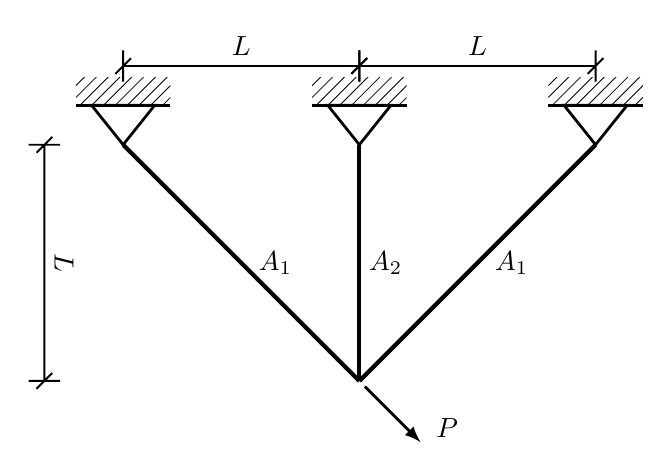
\begin{tikzpicture}
    \point{a}{0}{0};
    \point{b}{3}{0};
    \point{c}{6}{0};
    \point{d}{3}{-3};
    \beam{2}{a}{d};
    \beam{2}{b}{d};
    \beam{2}{c}{d};
    \support{1}{a}[180];
    \support{1}{b}[180];
    \support{1}{c}[180];
    \load{1}{d}[135][1][-1.1];
    \notation {1}{d}{$P$}[below right=5mm, xshift=5mm]; 
    \notation {5}{a}{d}[$A_1$][0.5][right, xshift=1mm][1];
    \notation {5}{b}{d}[$A_2$][0.5][right][1];
    \notation {5}{c}{d}[$A_1$][0.5][right, xshift=1mm][1];
    \dimensioning{1}{a}{b}{1}[$L$];
    \dimensioning{1}{b}{c}{1}[$L$];

    %\point{e}{0}{-3};
    \dimensioning{2}{a}{d}{-1}[$L$];

\end{tikzpicture}

\end{document}
